\chapter{Analysis Details}

\section{Multi-strange baryons}
Multi-strange baryons, possessing more than one strange quark, are of particular importance in the study of particle production mechanisms, as their dominant
strange quark content makes them susceptible to changes in hadrochemistry of the colliding systems. This analysis attempts to probe the multi-strange
baryon yields in proton-lead (p-Pb) collisions at centre-of-mass energy of $\sqrt{s_{\textnormal{\sc nn}}}$ = 8.16 TeV measured at the ALICE detector in
LHC. A total of six multi-strange baryons, including $\Xi^{0} (uss)$, $\Xi^{-} (dss)$, and $\Omega^{-} (sss)$, along with their corresponding antiparticles
$\bar{\Xi^{0}}$, $\bar{\Xi^{+}}$, and $\bar{\Omega^{+}}$ are of interest. They are known as cascade particles owing to their doubly weak decay mechanism.
Since the initial state colliding particles do not contain any strange valence quarks, all particles with a non-zero strangeness quantum number are
generated during the course of the collision. A summary of particles of interest along with their decay paths and branching ratios are tabulated in
Table \ref{tab:cascades}.

\begin{table}[H]
    \centering
    \begin{tabular}{|l|r|l|r|r|}
        \hline
        Particle                  & Mass (MeV/$c^{2}$)   & Decay Mode          & Branching Ratio (\%) & Lifetime $c\tau$ (cm) \\ \hline
        $\Xi^{0}$                 & $1314.86 \pm 0.20$   & $\Lambda \pi^{0}$   & $99.525 \pm 0.012$   & 8.71                  \\ \hline
        $\Xi^{\pm}$               & $1321.71 \pm 0.0.07$ & $\Lambda \pi^{\pm}$ & $99.887 \pm 0.035$   & 4.91                  \\ \hline
        $\Omega^{\pm}$            & $1672.45 \pm 0.29$   & $\Lambda K^{\pm}$   & $67.8 \pm 0.7$       & 2.461                 \\ \hline
        $\Lambda / \bar{\Lambda}$ & $1115.683 \pm 0.006$ & $p^{\pm} \pi^{\mp}$ & $63.9 \pm 0.05$      & 7.89                  \\ \hline
    \end{tabular}
    \caption{Cascade baryons and their properties\cite{Pdg:2018}}
    \label{tab:cascades}
\end{table}


The inner tracking detectors of the experimental setup in ALICE are capable of identifying only charged particles, and thus $\Xi^{0} (uss)$ which
predominantly decays through uncharged particles $\Xi^{0} \rightarrow \Lambda + \pi^{0}$ is not measured. Thus, this analysis is performed on
charged cascade candidates $\Xi^{-}$, $\Omega^{-}$, $\bar{\Xi^{+}}$, and $\bar{\Omega^{+}}$. The analysis involves initial event, track and cascade
candidate selection, signal extraction for transverse momentum ($p_{\textnormal{\sc t}}$) spectra, correcting for pileups, efficiency calculations
and corrected spectra, and evaluating systematic uncertainities.

\section{Reconstruction}
Given their short lifetime, the cascade particles travel a small distance $L$ (decay length) before they undergo a weak decay:

\begin{equation}
    L = \frac{p\tau}{m}
\end{equation}

where $p$ is the total momentum, $\tau$ refers to the proper lifetime and $m$ is mass of the particle. $\Xi^{\pm}$ ($\Omega^{\pm}$) primarily decay into a
$\Lambda$ baryon and $\pi^{\pm} (K^{\pm})$ (called
Bachelor). The $\Lambda$ baryon, being electrically neutral, cannot be tracked by the detector. However, it further decays into a $p^{+} \pi^{-}$ pair
which, possessing electric charge, can be identified. Because of its distinctive "V" shape of the decay vertex generating two oppositely charged particles,
the neutral $\Lambda$ is characterised as V0. The decay topology can be seen in Fig. \ref{fig:cascDecay}.


\begin{figure}[H]
    \centering
    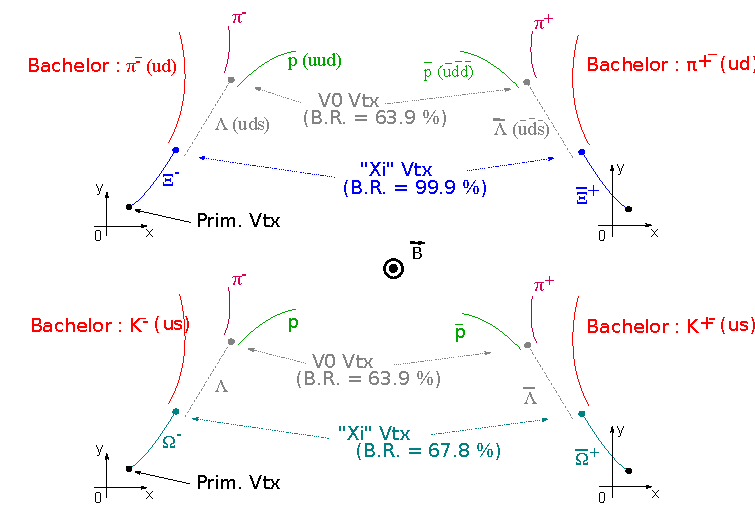
\includegraphics[width=0.75\linewidth]{images/cascDecay.pdf}
    \\
    \caption{Decay topology for charged cascade candidates $\Xi^{\pm}$ and $\Omega^{\pm}$\cite{Maire:2011}}
    \label{fig:cascDecay}
\end{figure}

The short decay length of the cascades is insufficient for direct observations in the ITS (with the closest SPD layer 3.9 cm from the interaction point).
Therefore, the cascade candidates are reconstructed with the help of the charged bachelor tracks and V0 daughter tracks. A two-step reconstruction
procedure employing $\Lambda$ reconstruction from the V0 daughter tracks and cascade candidate reconstruction using the reconstructed $\Lambda$ and an
associated bachelor track is implemented. Various kinematic and geometric selection criteria based on the decay topologies are used for deciding the
cascade candidates and eliminating combinatorial background, as outlined in Section \ref{sec:casc}.

\section{Data Sample}
The analysis is conducted on data obtained from proton-lead (p-Pb) collisions at $\sqrt{s_{\textnormal{\sc nn}}}$ = 8.16 TeV collected by the ALICE detector during
LHC's Run 2 phase in 2016. The particular dataset used for the analysis is internally referred to as "LHC16r\_pass2 \_CENT\_wSDD". The current analysis has been
performed on 6 runs marked as 'Good' in the Run Coordination Table: 265594, 265596, 265607, 266316, 266317 and 266318. They have been selected because of
relatively low interaction rates (<50 kHz) indicating low out-of-bunch pileup. These runs represent about 40\% of the total statistics available for this
period. The full processed statistics for the analysis comprises of $15.7 \times 10^{6}$ events.

The data sample is available as AOD files on CERN's computing network. The analysis code is written in CERN's software framework for data analysis: ROOT 6,
in conjunction with AliRoot libraries from the ALICE team. The analysis was performed on CERN's GRID network.

\section{Event selection criteria}

Basic event selection criteria following ALICE convention for p-Pb collisions were applied in this analysis. The event selection performed include $\colon$

\begin{itemize}
    \item \textbf{Minimum-bias trigger}: The minimum bias trigger aims to select only inelastic events, excluding collisions with residual gas in the beam pipe.
          This requires at least one hit (non-zero signal) in the VZERO detector on both sides of the collision (VZERO-A and VZERO-C).
    \item \textbf{Primary Vertex position}: Events with primary vertex within $|z|<10$ cm from the center of the detector along the $z$-axis were chosen.
    \item \textbf{INEL>0 event selection}: Only events with at least one reconstructed SPD tracklet in the $|\eta|$ < 1.0 range were selected for analysis.
    \item \textbf{Event multiplicity selection}: Due to the assymetric nature of the collision, the multiplicity estimator based on the VZERO-A amplitude was
          selected (Pb-going direction).
\end{itemize}

Moreover, event multiplicity classes to maximise the multplicity bins that could be explored with the present statistics were chosen. The classes are
enlisted in Table \ref{tab:multi}, with 0-5\% representing the highest multiplicities and 80-100\% ($\Xi^{\pm}$) or 60-100\% ($\Omega^{\pm}$) representing
the lowest multiplicities.

\begin{table}[H]
    \centering
    \begin{tabular}{|l|l|}
        \hline
        \textbf{Particle} & \textbf{V0A multiplicity classes (\%)}                             \\ \hline
        $\Xi^{\pm}$       & 0-5, 5-10, 10-15, 15-20, 20-30, 30-40, 40-50, 50-60, 60-80, 80-100 \\ \hline
        $\Omega^{\pm}$    & 0-5, 5-15, 15-30, 30-60, 60-100                                    \\ \hline
    \end{tabular}
    \caption{V0A multiplicity classes for cascades}
    \label{tab:multi}
\end{table}
The remaining sample after application of aforementioned event selection criteria had $11.2 \times 10^{6}$ events.

\section{Cascade candidates selection}\label{sec:casc}

Cascade candidate selection based on the decay topology were applied to ensure geometrical characteristics of the tracks comply with expected decay
mechanism. Some topological variables are illustrated in Fig. \ref{fig:topo}.

\begin{figure}[H]
    \centering
    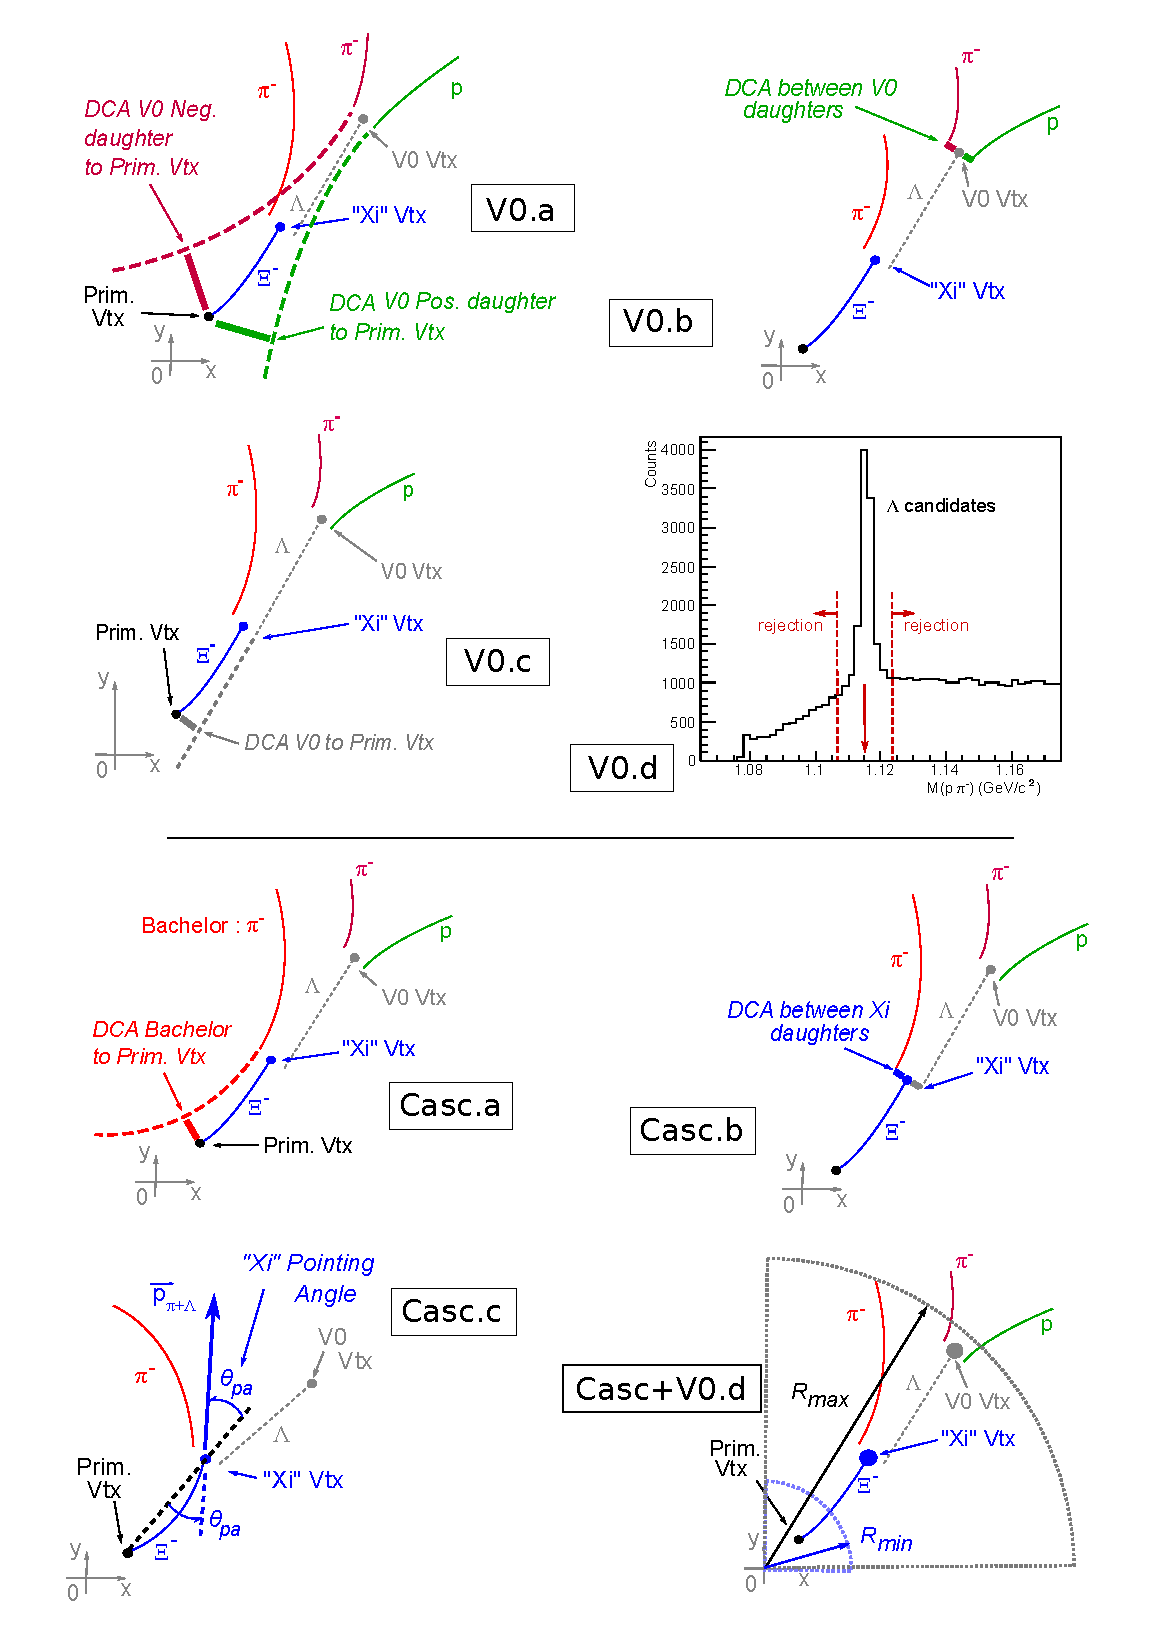
\includegraphics[clip,trim={0 0 0 14.3cm}, width=0.75\linewidth]{images/topologoical.pdf}
    \\
    \caption{Topological variables for cascades\cite{MaireTop:2011}}
    \label{fig:topo}
\end{figure}

\begin{itemize}
    \item \textbf{Rapidity interval}: The chosen rapidity interval for the analysis is -0.5 < y <0 corresponding to central rapidity region in p-Pb
          collisions.
    \item \textbf{Proper lifetime}: A proper lifetime selection of $\frac{mL}{p} < 3\times c\tau$ is applied, where $m$ denotes the cascade mass, $L$ is the
          cascade's decay length, $p$ is its total momentum and $c\tau$ is the lifetime (values in Table \ref{tab:cascades}). This helps to remove track combinations
          from low-momentum candidates originating unusually far from the Primary Vertex (PV).
    \item \textbf{TPC $\textbf{d}E/\textbf{d}x$ selection}: A cut on TPC's energy loss $\textnormal{d}E/\textnormal{d}x$
          is applied to remove background combinations of tracks from wrong particle species. Acceptance range of $4\sigma$
          is tolerated for cascade candidate's three daughter tracks.
    \item \textbf{Competing cascade rejection}: There is a significant background contribution from $\Xi^{\pm}$ decays
          while conducting the $\Omega^{\pm}$ analyses. To eliminate this background, it is necessary for the mass under
          $\Xi^{\pm}$ hypothesis to differ by at least 8 MeV/$c^{2}$ from the corresponding PDG mass.

    \item \textbf{Number of TPC clusters}: A minimum of 70 TPC clusters requirement is imposed to select good quality tracks.

\end{itemize}

All selection criteria involved in this analysis are listed in Table \ref{tab:crit}.

\begin{table}[H]
    \centering
    \begin{tabular}{|l|r|}
        \hline
        \textbf{Topological Variable}                          & \textbf{$\Xi (\Omega)$ Cut}             \\
                                                               & low, mid, high $p_{\textnormal{\sc t}}$ \\ \hline
        \hline

        Cascade transv. decay radius $R_{\textnormal{\sc 2d}}$ & >0.6 (0.5) cm                           \\ \hline
        V0 transv. decay radius                                & >1.2 (1.1) cm                           \\ \hline
        DCA (bachelor - PV)                                    & >0.04 cm                                \\ \hline
        DCA (V0 - PV)                                          & >0.06 cm                                \\ \hline
        DCA (meson V0 track - PV)                              & >0.04 cm                                \\ \hline
        DCA (baryon V0 track  - PV)                            & >0.03 cm                                \\ \hline
        DCA (V0 tracks)                                        & <1.7, 1.6, 1.5 $\sigma$                 \\ \hline
        DCA (bachelor - V0)                                    & <1.6, 1.5, 1.4 cm                       \\ \hline
        Cascade $\cos(PA)$                                     & >0.96, 0.97, 0.97                       \\ \hline
        V0 $\cos(PA)$                                          & >0.98 (0.97, 0.98, 0.98)                \\ \hline
        V0 invariant mass window                               & $\pm 0.008$ GeV/$c^{2}$                 \\ \hline
        \hline
        \textbf{Selection}                                     & \textbf{$\Xi (\Omega)$ Cut}             \\ \hline
        \hline
        Rapidity Interval                                      & -0.5 < $y$ < 0                          \\ \hline
        TPC $\textnormal{d}E/\textnormal{d}x$ selection        & < 4$\sigma$                             \\ \hline
        Proper lifetime ($\frac{mL}{p}$)                       & $< 3\times c\tau$                       \\ \hline
        Daughter Track $N_{\textnormal{TPC clusters}}$         & $\geq$ 70                               \\ \hline
        Competing cascade rejection (only $\Omega$)            & $|M(\Xi)-1.321| > $ 8 MeV/$c^{2}$       \\ \hline
        Tracking flags for daughters                           & kTPCrefit                               \\ \hline
    \end{tabular}
    \caption{Selection criteria for $\Xi^{\pm}$ and $\Omega^{\pm}$ candidates}
    \label{tab:crit}
\end{table}

The $p_{\textnormal{\sc t}}$ bin ranges used for the analysis divided into low, mid and high $p_{\textnormal{\sc t}}$ categories are listed in Table \ref{tab:pt}:

\begin{table}[H]
    \centering
    \begin{tabular}{|l||r|r|r|}
        \hline
        \multirow{2}{*}{\textbf{Particle}} & \multicolumn{3}{c|}{\textbf{$p_{\textnormal{\sc t}}$ bins (GeV/$c$)}}                                                         \\ \cline{2-4}

                                           & Low                                                                   & Mid                         & High                    \\ \hline \hline
        $\Xi^{\pm}$                        & \{0.8,1.1,1.3,1.5,1.7,1.9\}                                           & \{1.9,2.1,2.3,2.5,2.7,2.9\} & \{2.9,3.1,3.5,4.0,5.5\} \\ \hline
        $\Omega^{\pm}$                     & \{0.9,1.6,2.0\}                                                       & \{2.0,2.4,2.9\}             & \{2.9,3.5,5\}           \\ \hline
    \end{tabular}
    \caption{$p_{\textnormal{\sc t}}$ bin ranges used in analysis}
    \label{tab:pt}
\end{table}

\section{Signal Extraction}
Cascade invariant mass is calculated according to multiplicity classes and transverse momentum ranges for signal extraction. The $p_{\textnormal{\sc t}}$
bin ranges used allow for a spread of $p_{\textnormal{\sc t}}$ to be observed yet making sure that enough statistics are available for good signal extraction.
Table \ref{tab:pt} lists the momentum bin ranges while table \ref{tab:multi} lists the multiplicity classes. The binning for momentum ranges does not start
at zero since low momentum cascade decay particles, having lower radius of curvature, fail to traverse the detectors and hence, are not measured.
Particle-antiparticle
combinations have also been plotted for better statistics alongside singular particle plots, and  they are consistent with each other while improving
fitting characteristics in ranges with low statistics.

Thus, invariant mass plots are generated for each multiplicity and $p_{\textnormal{\sc t}}$ bin. In order to extract signal from the plots, the signal
region is fitted with a Gaussian + $2^{nd}$ degree polynomial fit and peak mean ($\mu$) and width($\sigma$) are estimated. Knowing these parameters,
the signal region, also known as the peak window, can be defined. For this analysis, the peak window was deduced to be:

\begin{equation}
    (M-4\sigma) \to (M+4\sigma)
\end{equation}


where $M$ is the position of peak($\mu$) value, denoting the particle mass, and is in agreement with the PDG mass. In the signal region, bin counting
technique is used to sum up signal + background counts.

For background estimation, a linear fit was chosen owing to a mostly flat background curve. The interval chosen for linear fitting of the background is
wider than the peak window and excludes the signal region completely:

\begin{equation}
    (M-8\sigma) \to (M-4\sigma) \  ; \    (M+4\sigma) \to (M+8\sigma)
\end{equation}

This two-part fitting interval lies outside the signal region and gives a more accurate background estimation curve, especially in case of low statistics.
This background fit is then integrated in the signal region, i.e. $(M-4\sigma) \to (M+4\sigma)$, in order to calculate background contribution
to the signal peak. Finally, the signal extraction is achieved by subtracting the value of this background fit integral calculated for area under the peak
from the bin counting of signal + background in the peak window. Figure \ref{fig:sigeg} gives an example of signal extraction performed on the invariant
mass spectra for $\Xi^{+}$ and $\Omega^{-}$.

\begin{figure}[H]
    \centering
    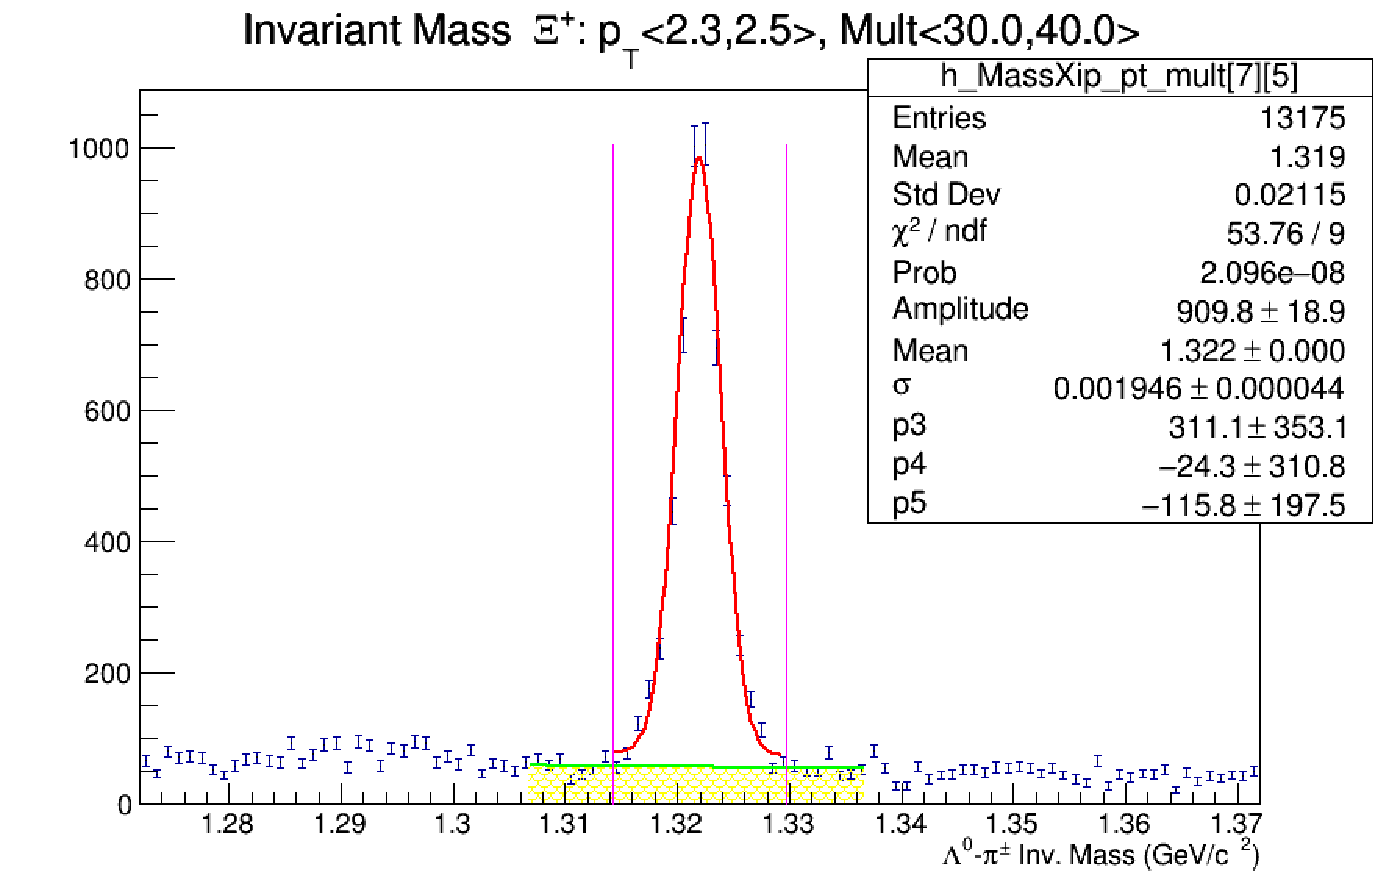
\includegraphics[width=0.75\linewidth]{images/xip_7_5.pdf}
    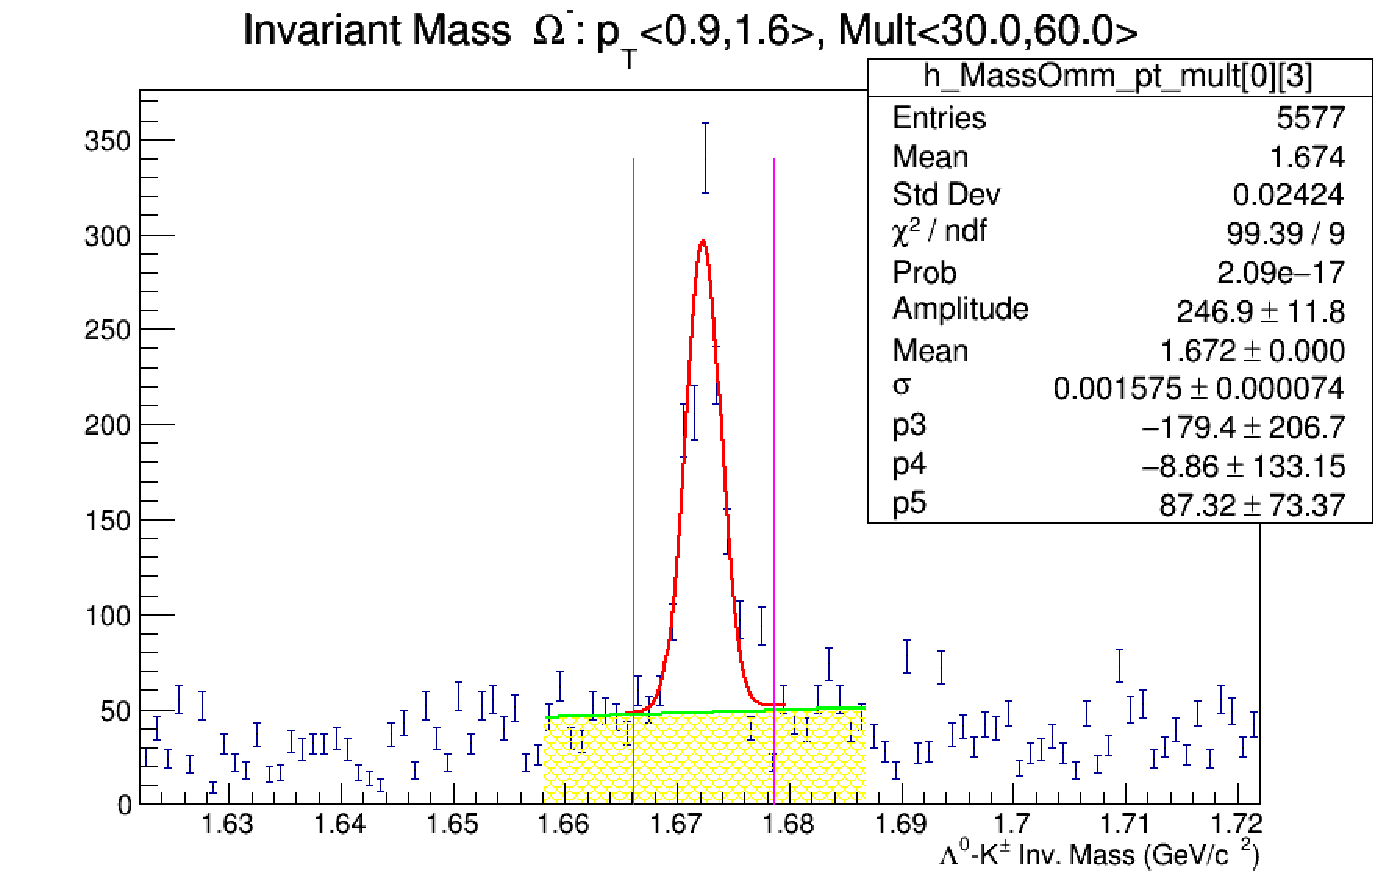
\includegraphics[width=0.75\linewidth]{images/omm_0_3.pdf}
    \caption{Plots showing examples of invariant mass for $\Xi^{+}$ (top) and $\Omega^{-}$ (bottom). $y$-axis denotes counts.}
    \label{fig:sigeg}
\end{figure}

In Figure \ref{fig:sigeg}, the red curve denotes Gaussian + $2^{nd}$ degree polynomial fit for the signal and the green curve denotes the linear fit of the
background, fitted for the region beyond the magenta lines. The peak window is encapsulated by the two vertical magenta lines. For background subtraction,
the area highlighted in yellow under the peak is used, limited by the vertical magenta lines.

\section{Raw transverse momentum spectra}

Using the procedure mentioned in the previous section, raw transverse momentum spectra ($p_{\textnormal{\sc t}}$) for $\Xi^{\pm}$ and $\Omega^{\pm}$ along
with particle anti-particle combination spectra were obtained and are shown in figure \ref{fig:rawpt} for different V0A multiplicity classes.

\begin{figure}[H]
    \centering
    \begin{subfigure}{.5\textwidth}
        \centering
        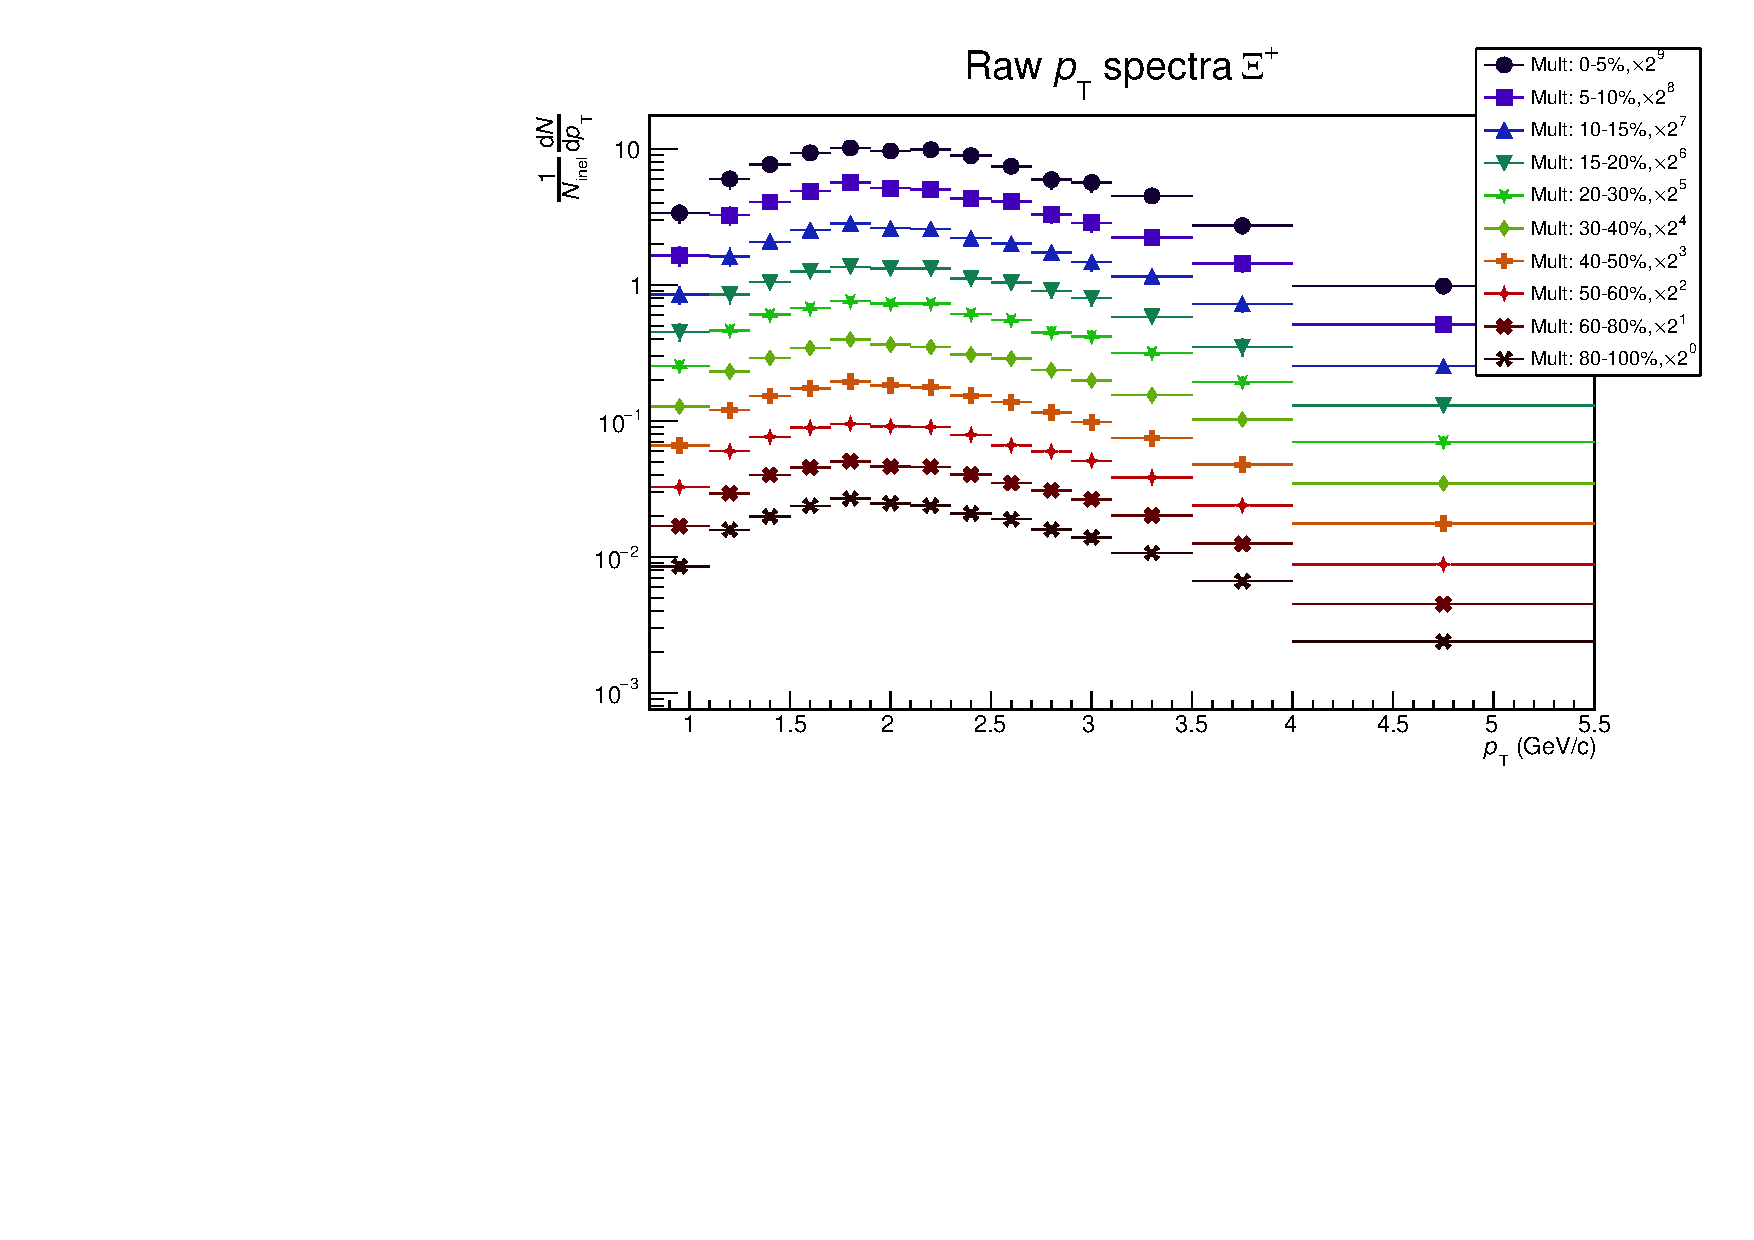
\includegraphics[width=\linewidth]{images/raw_xip.pdf}
    \end{subfigure}%
    \begin{subfigure}{.5\textwidth}
        \centering
        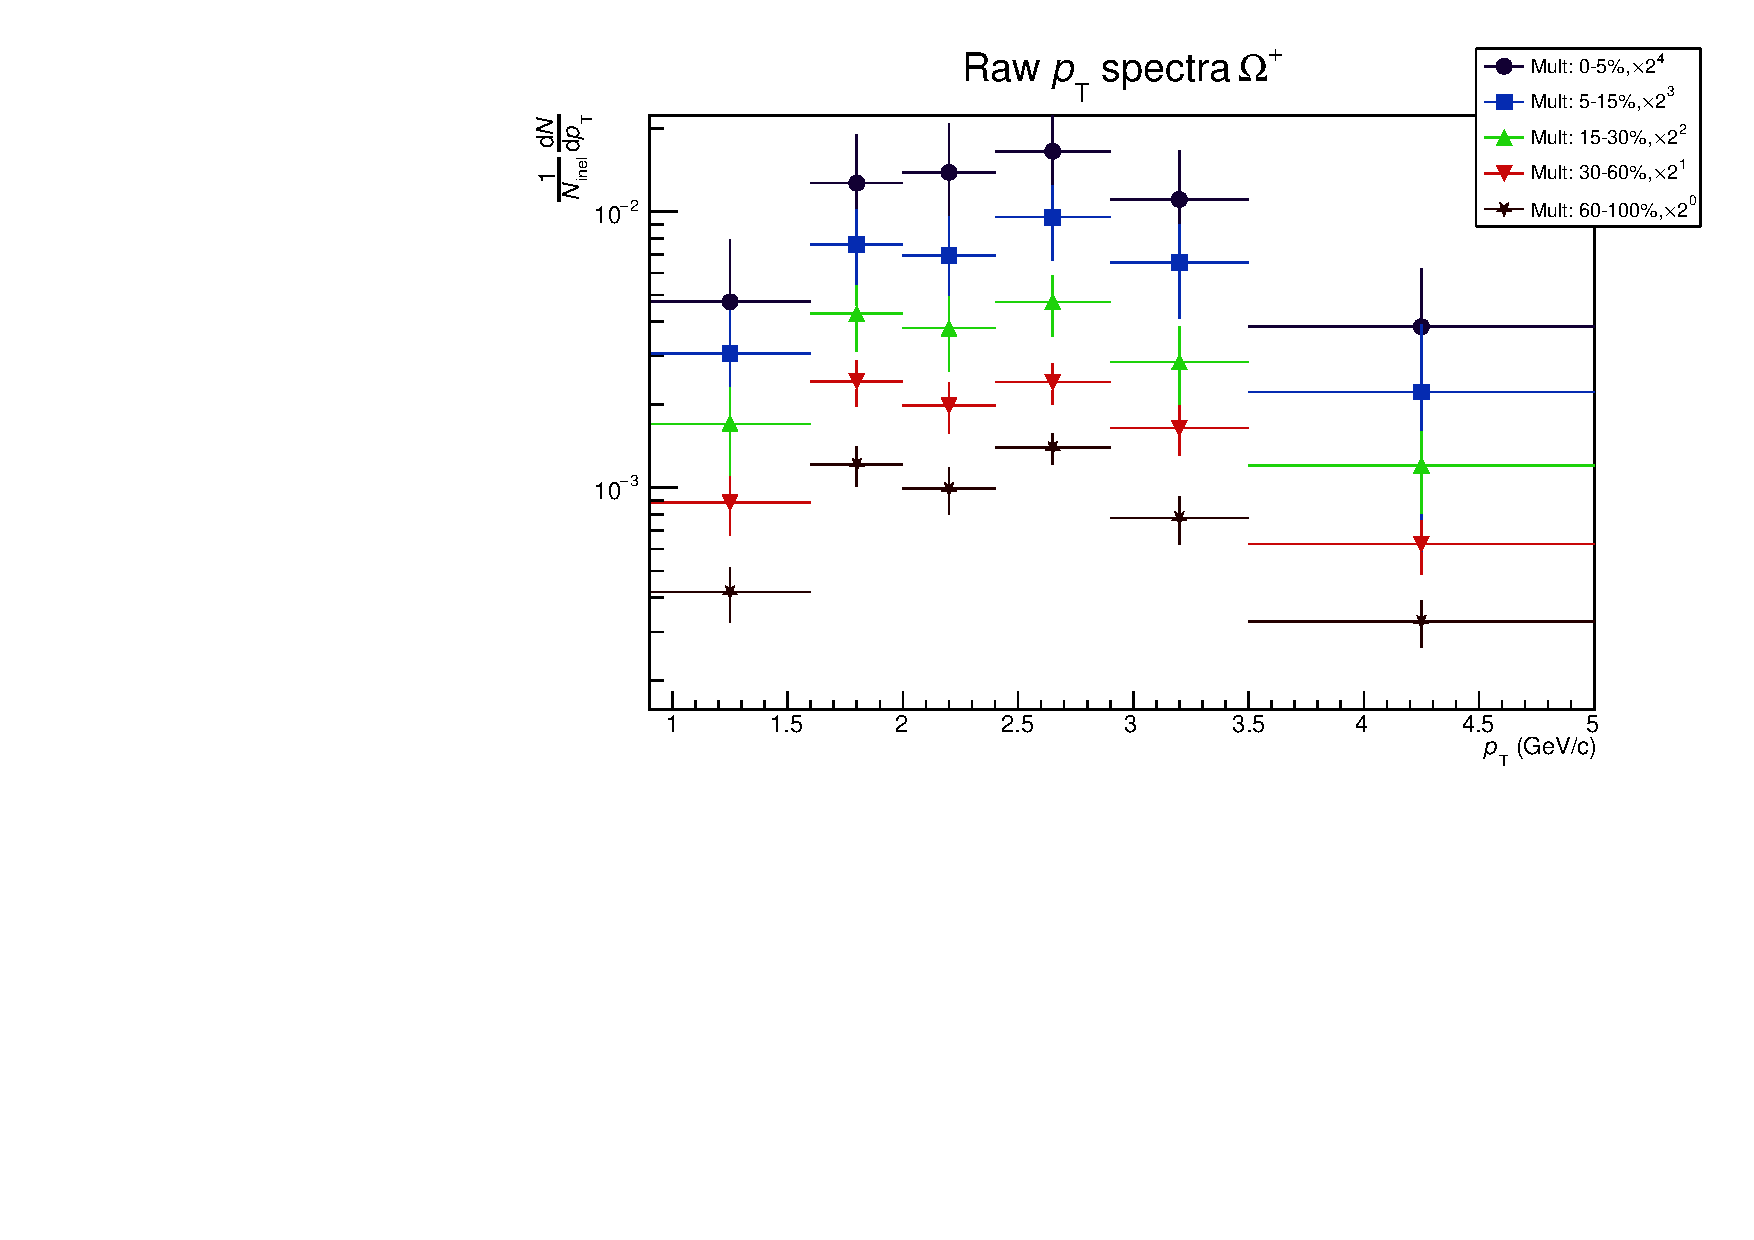
\includegraphics[width=\linewidth]{images/raw_omp.pdf}
    \end{subfigure}

    \medskip
    \begin{subfigure}{.5\textwidth}
        \centering
        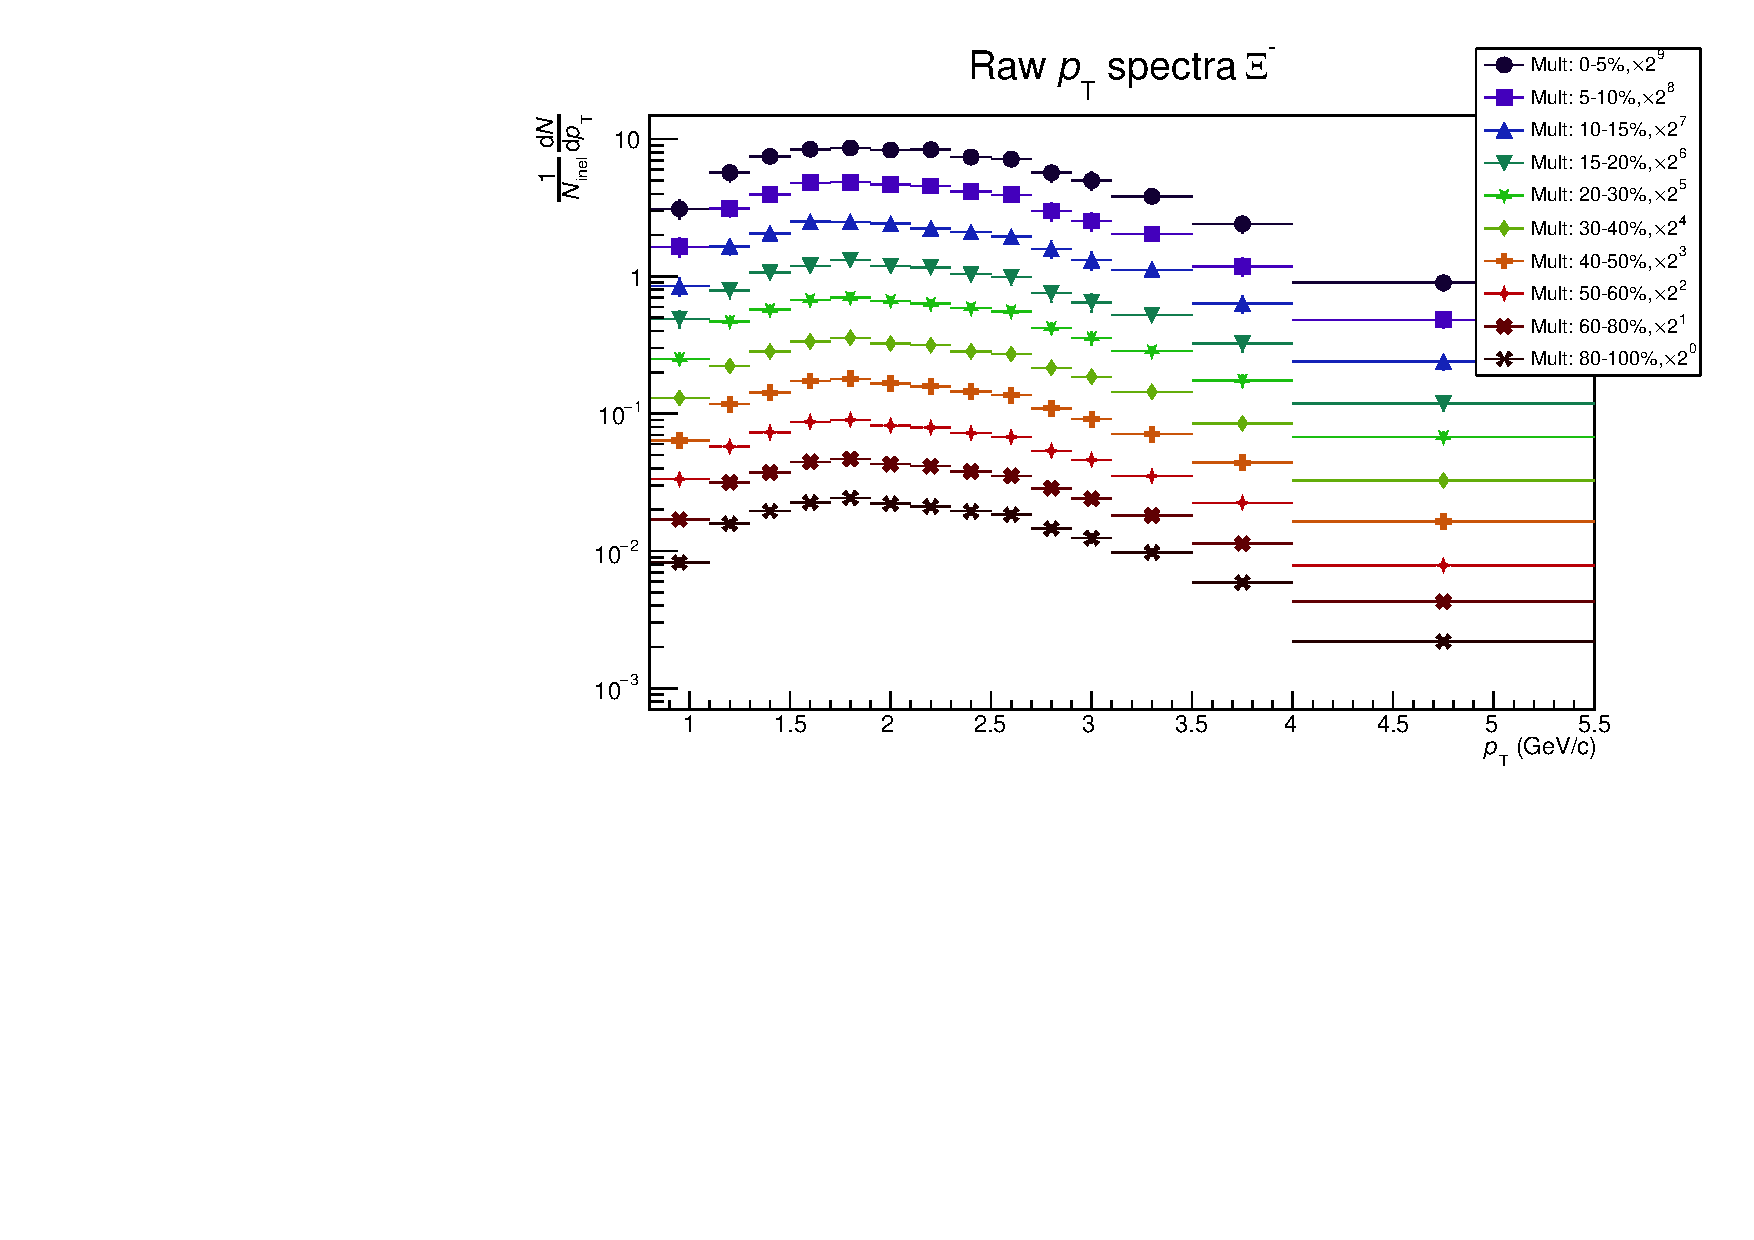
\includegraphics[width=\linewidth]{images/raw_xim.pdf}
    \end{subfigure}%
    \begin{subfigure}{.5\textwidth}
        \centering
        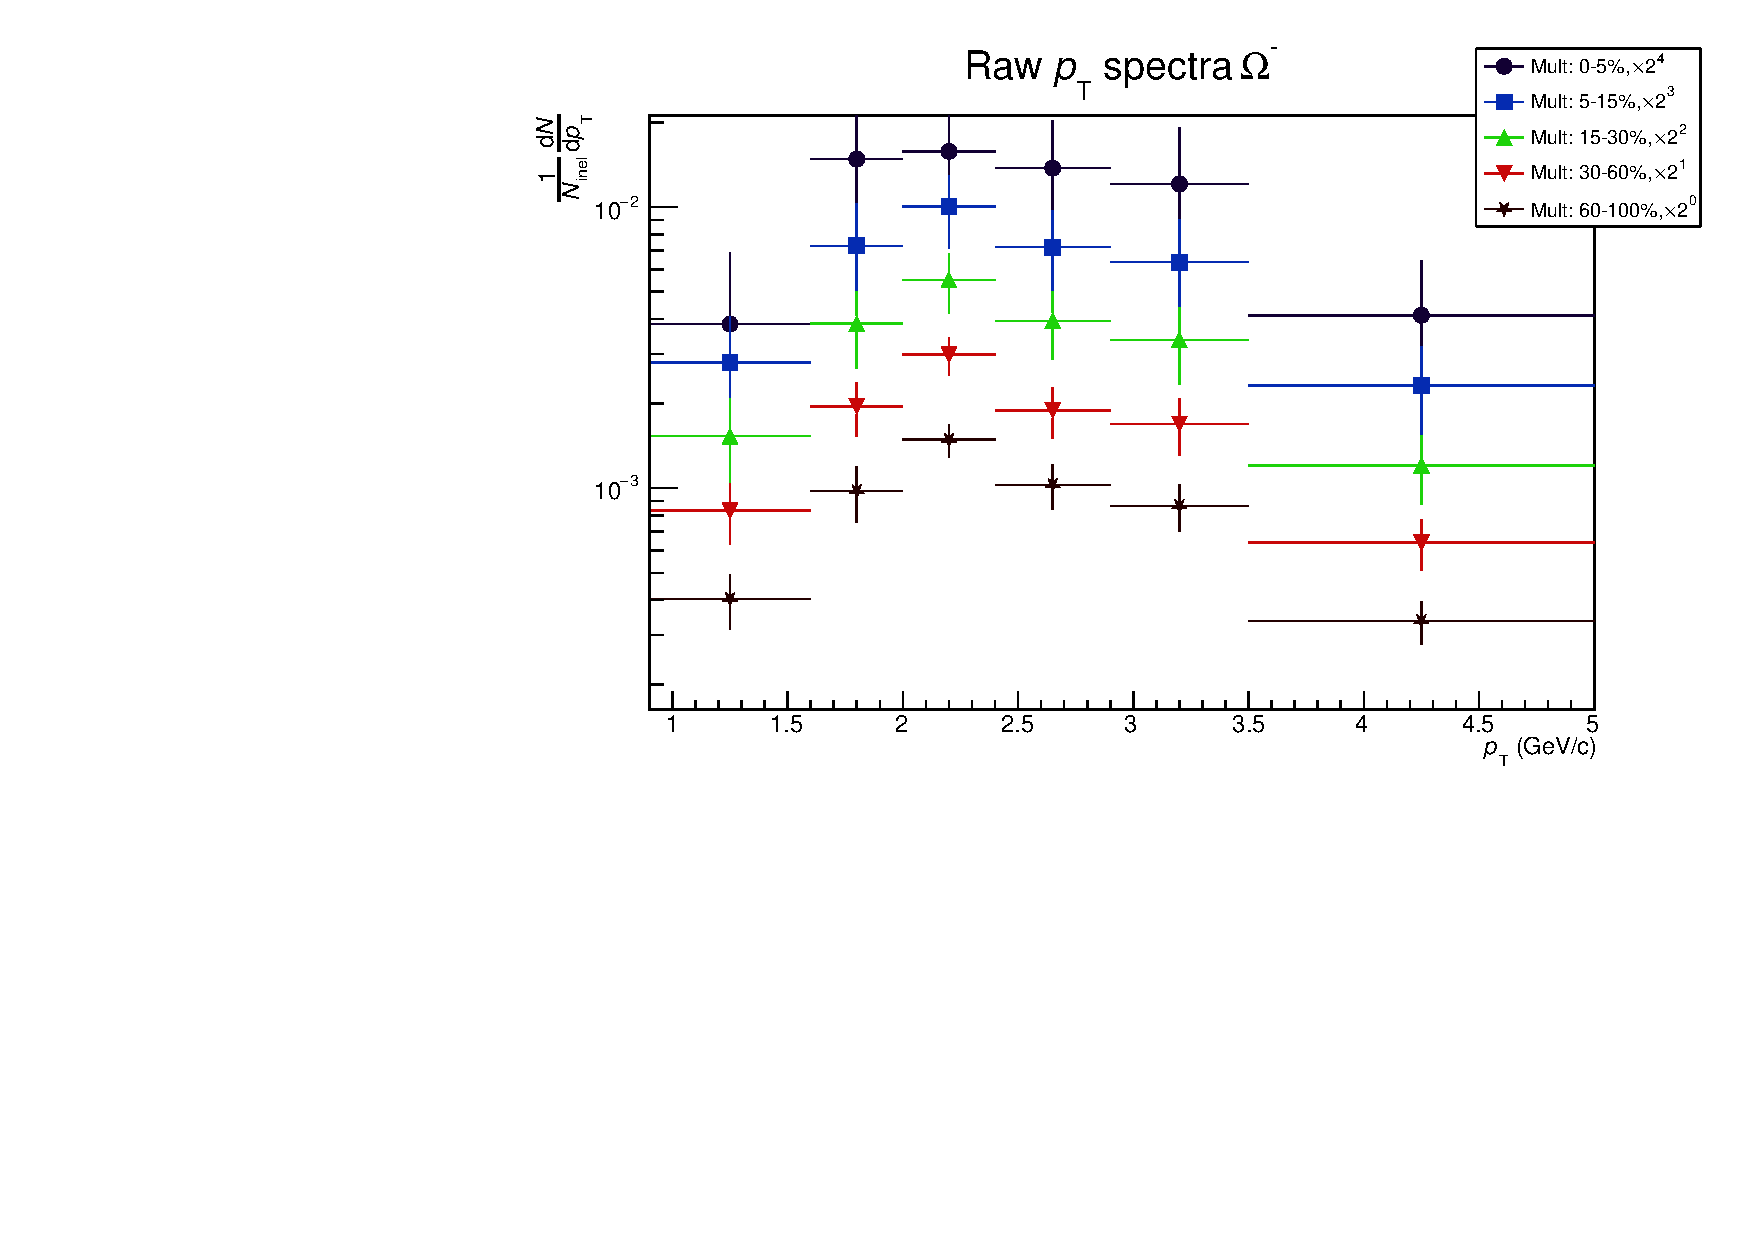
\includegraphics[width=\linewidth]{images/raw_omm.pdf}
    \end{subfigure}

    \medskip
    \begin{subfigure}{.5\textwidth}
        \centering
        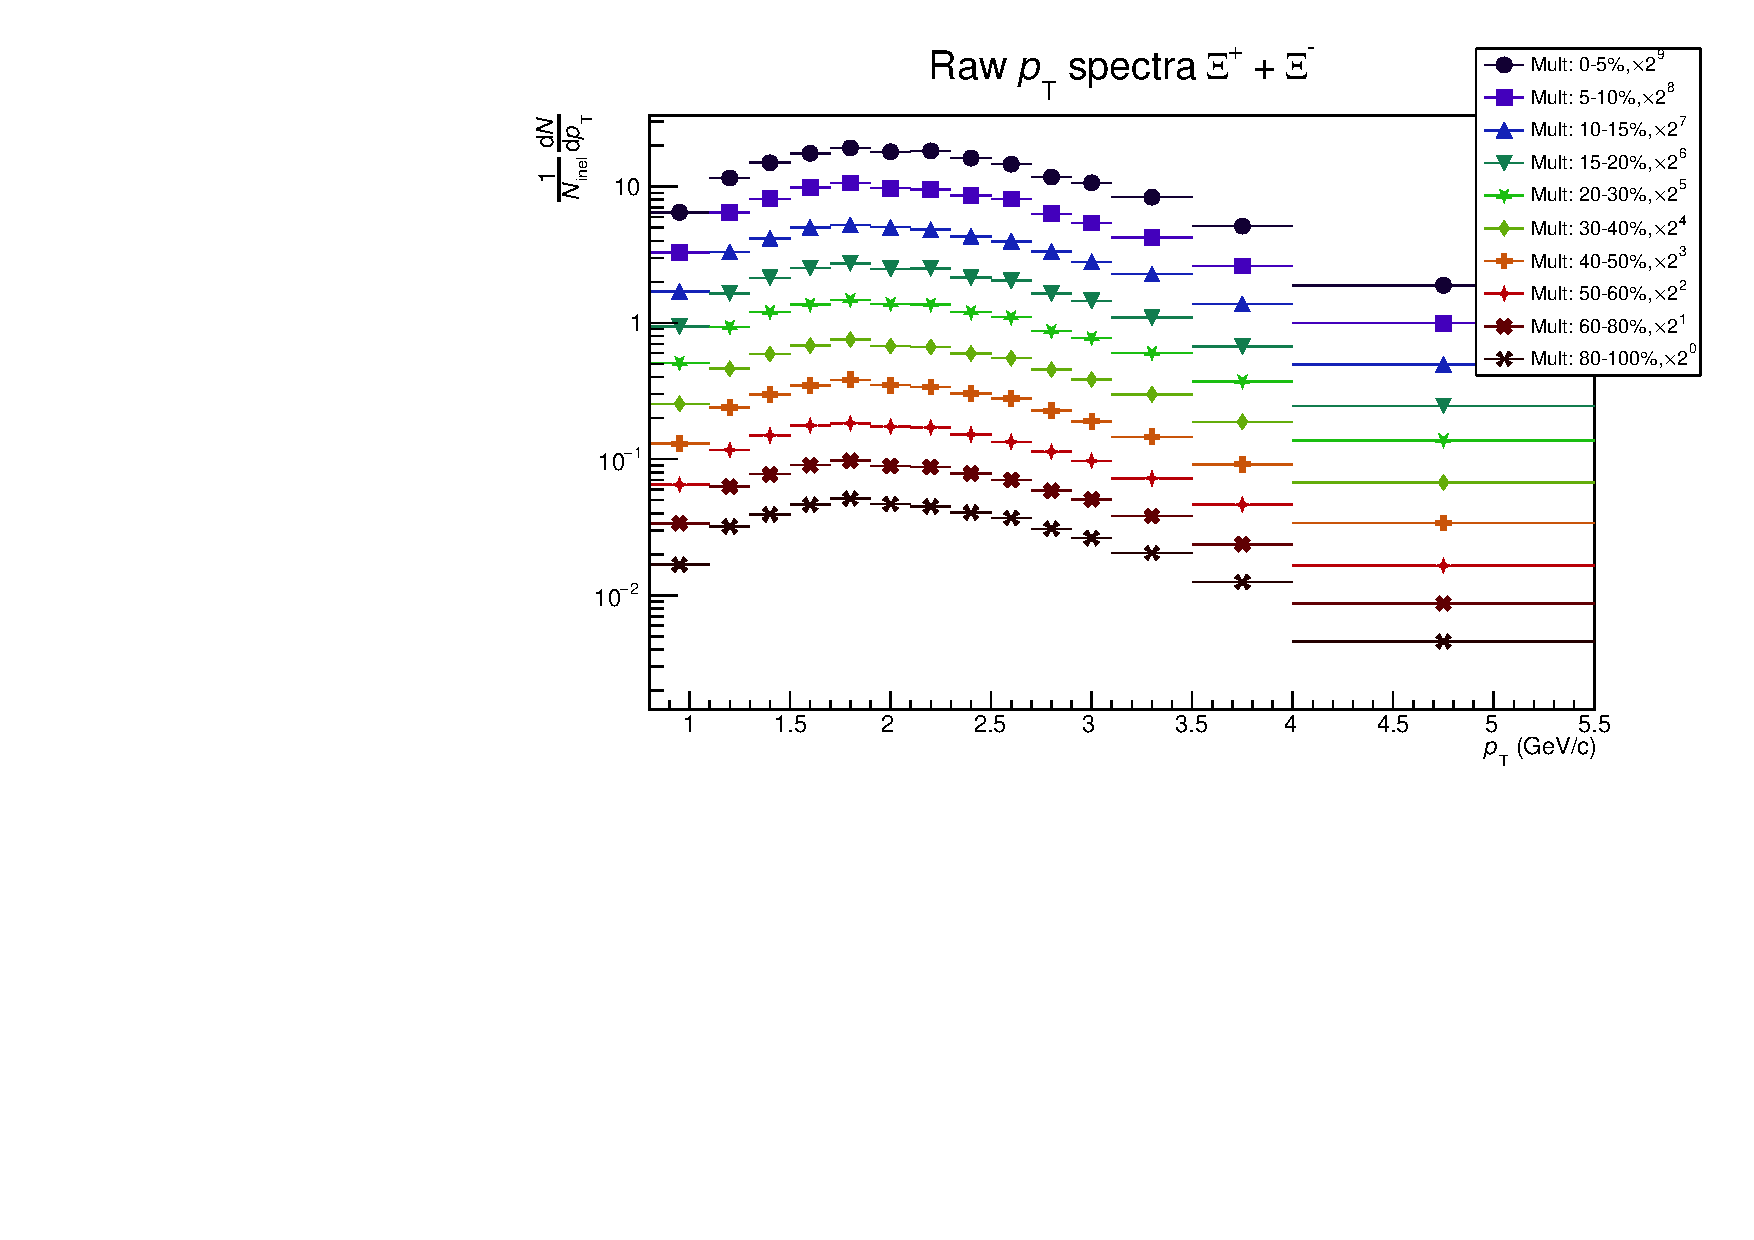
\includegraphics[width=\linewidth]{images/raw_xiC.pdf}
    \end{subfigure}%
    \begin{subfigure}{.5\textwidth}
        \centering
        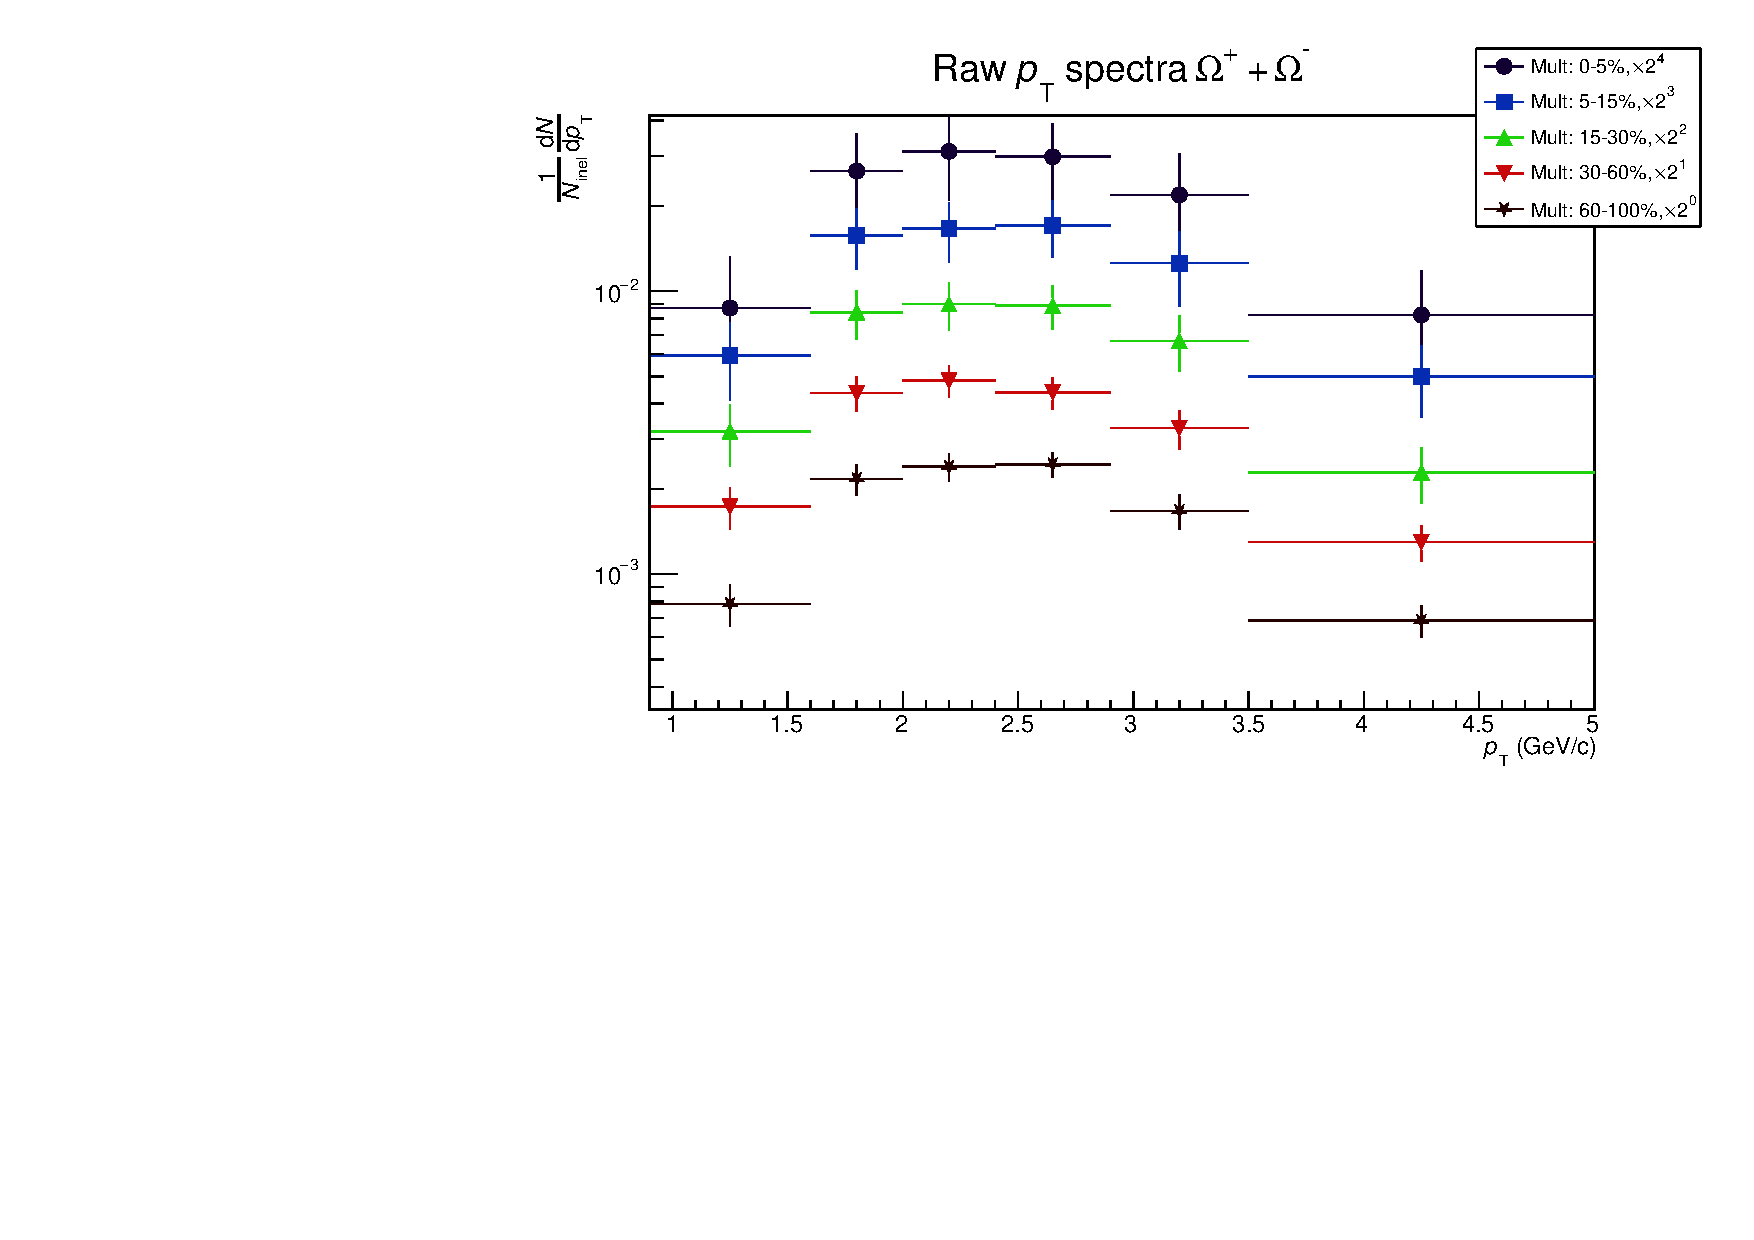
\includegraphics[width=\linewidth]{images/raw_omC.pdf}
    \end{subfigure}
    \caption{Plots depicting raw ($p_{\textnormal{\sc t}}$) spectra for $\Xi^{\pm}$ (left) and $\Omega^{\pm}$ (right)}
    \label{fig:rawpt}
\end{figure}

In figure \ref{fig:rawpt}, the left side denotes the raw transverse momentum spectra for $\Xi^{\pm}$ and the right side for $\Omega^{\pm}$. The top
figures are for the positively charged particle spectra, middle for negatively charged and the bottom ones as a combination of the two.